\documentclass[UTF8,a4paper,11pt]{ctexart}

\usepackage{amsmath}
\usepackage{booktabs}
\usepackage{geometry}
\usepackage{graphicx}
\usepackage{caption}
\usepackage{float}
\usepackage{hyperref}

\geometry{left=2.5cm,right=2.5cm,top=2.5cm,bottom=2.5cm}
\hypersetup{colorlinks=true,linkcolor=black,urlcolor=blue}
\captionsetup{font=small}

\title{Model A 数值模拟实验报告}
\author{MSWD Bootstrapping Reproduction}
\date{\today}

\begin{document}
\maketitle

\section{实验设置}

本报告基于根目录下由 \texttt{main.py} 生成的控制台日志文件：
\[
\texttt{results\_beta*.txt}.
\]
这些日志来自命令形式：
\[
\texttt{python -u main.py --signal <value> >> results\_beta*.txt}.
\]

由于同一参数下可能分多次运行，例如 \texttt{results\_beta0\_1.txt}、
\texttt{results\_beta0\_2.txt} 等，每个文件内部的累计拒绝率都从 \texttt{run 0}
重新开始。因此统计时没有直接拼接日志中的累计拒绝率，而是先在每个文件内部按完整轮次统计拒绝次数，再按该文件贡献的完整轮数进行加权合并。

完整轮次的判定标准为该轮已经输出到 \texttt{main.py} 默认流程的最后一个方法：
\[
\texttt{run k, percentage of rejection: pwd perm k3 ...}.
\]
每个参数只保留前 50 个完整轮次，超过 50 的轮次不纳入本报告统计。

本次绘图包含日志中可以可靠恢复的五种方法：
\[
\text{Proposed},\quad \text{MMD-G},\quad \text{ED2},\quad \text{BG},\quad \text{PW}.
\]
需要说明的是，虽然 \texttt{permTest.py} 内部计算了 Laplace kernel MMD 的
\texttt{lapmmd\_decision}，但是 \texttt{main.py} 的日志没有打印该结果，因此无法从已有
\texttt{txt} 日志中恢复论文图中的 \text{MMD-L} 曲线。

\section{Model A 设置}

本实验采用 \texttt{main.py} 的默认模型 \texttt{mean-decay}。在代码中，两组样本满足：
\[
X \sim N(0_p, \Sigma), \qquad
Y \sim N(\mu, \Sigma),
\]
其中协方差矩阵为 Toeplitz 相关结构：
\[
\Sigma_{ij}=0.5^{|i-j|}.
\]
均值差异按照坐标衰减：
\[
\mu_j = \frac{\texttt{signal}}{j^3}, \qquad j=1,\ldots,p.
\]

本次日志文件名中的 \(\beta\) 与运行时传入的 \texttt{signal} 对应，即横轴取：
\[
\beta \in \{0, 0.2, 0.4, 0.6, 0.8, 1.0\}.
\]

主要默认参数为：
\[
n_1=250,\quad n_2=250,\quad p=500,\quad \alpha=0.05.
\]
Proposed 方法对应 L0 sparse max-sliced Wasserstein distance 与 bootstrap 检验。

\section{实验结果}

表 \ref{tab:result} 给出了每个 \(\beta\) 下前 50 个完整轮次的经验拒绝率。

\begin{table}[H]
\centering
\caption{Model A 下前 50 个完整轮次的经验拒绝率}
\label{tab:result}
\begin{tabular}{cccccc}
\toprule
\(\beta\) & Proposed & MMD-G & ED2 & BG & PW \\
\midrule
0.0 & 0.08 & 0.02 & 0.02 & 0.00 & 0.04 \\
0.2 & 0.06 & 0.02 & 0.02 & 0.02 & 0.06 \\
0.4 & 0.28 & 0.18 & 0.18 & 0.06 & 0.08 \\
0.6 & 0.84 & 0.08 & 0.08 & 0.02 & 0.08 \\
0.8 & 0.98 & 0.26 & 0.30 & 0.02 & 0.14 \\
1.0 & 1.00 & 0.58 & 0.56 & 0.08 & 0.24 \\
\bottomrule
\end{tabular}
\end{table}

图 \ref{fig:modela} 展示了对应的经验拒绝率曲线。

\begin{figure}[H]
\centering
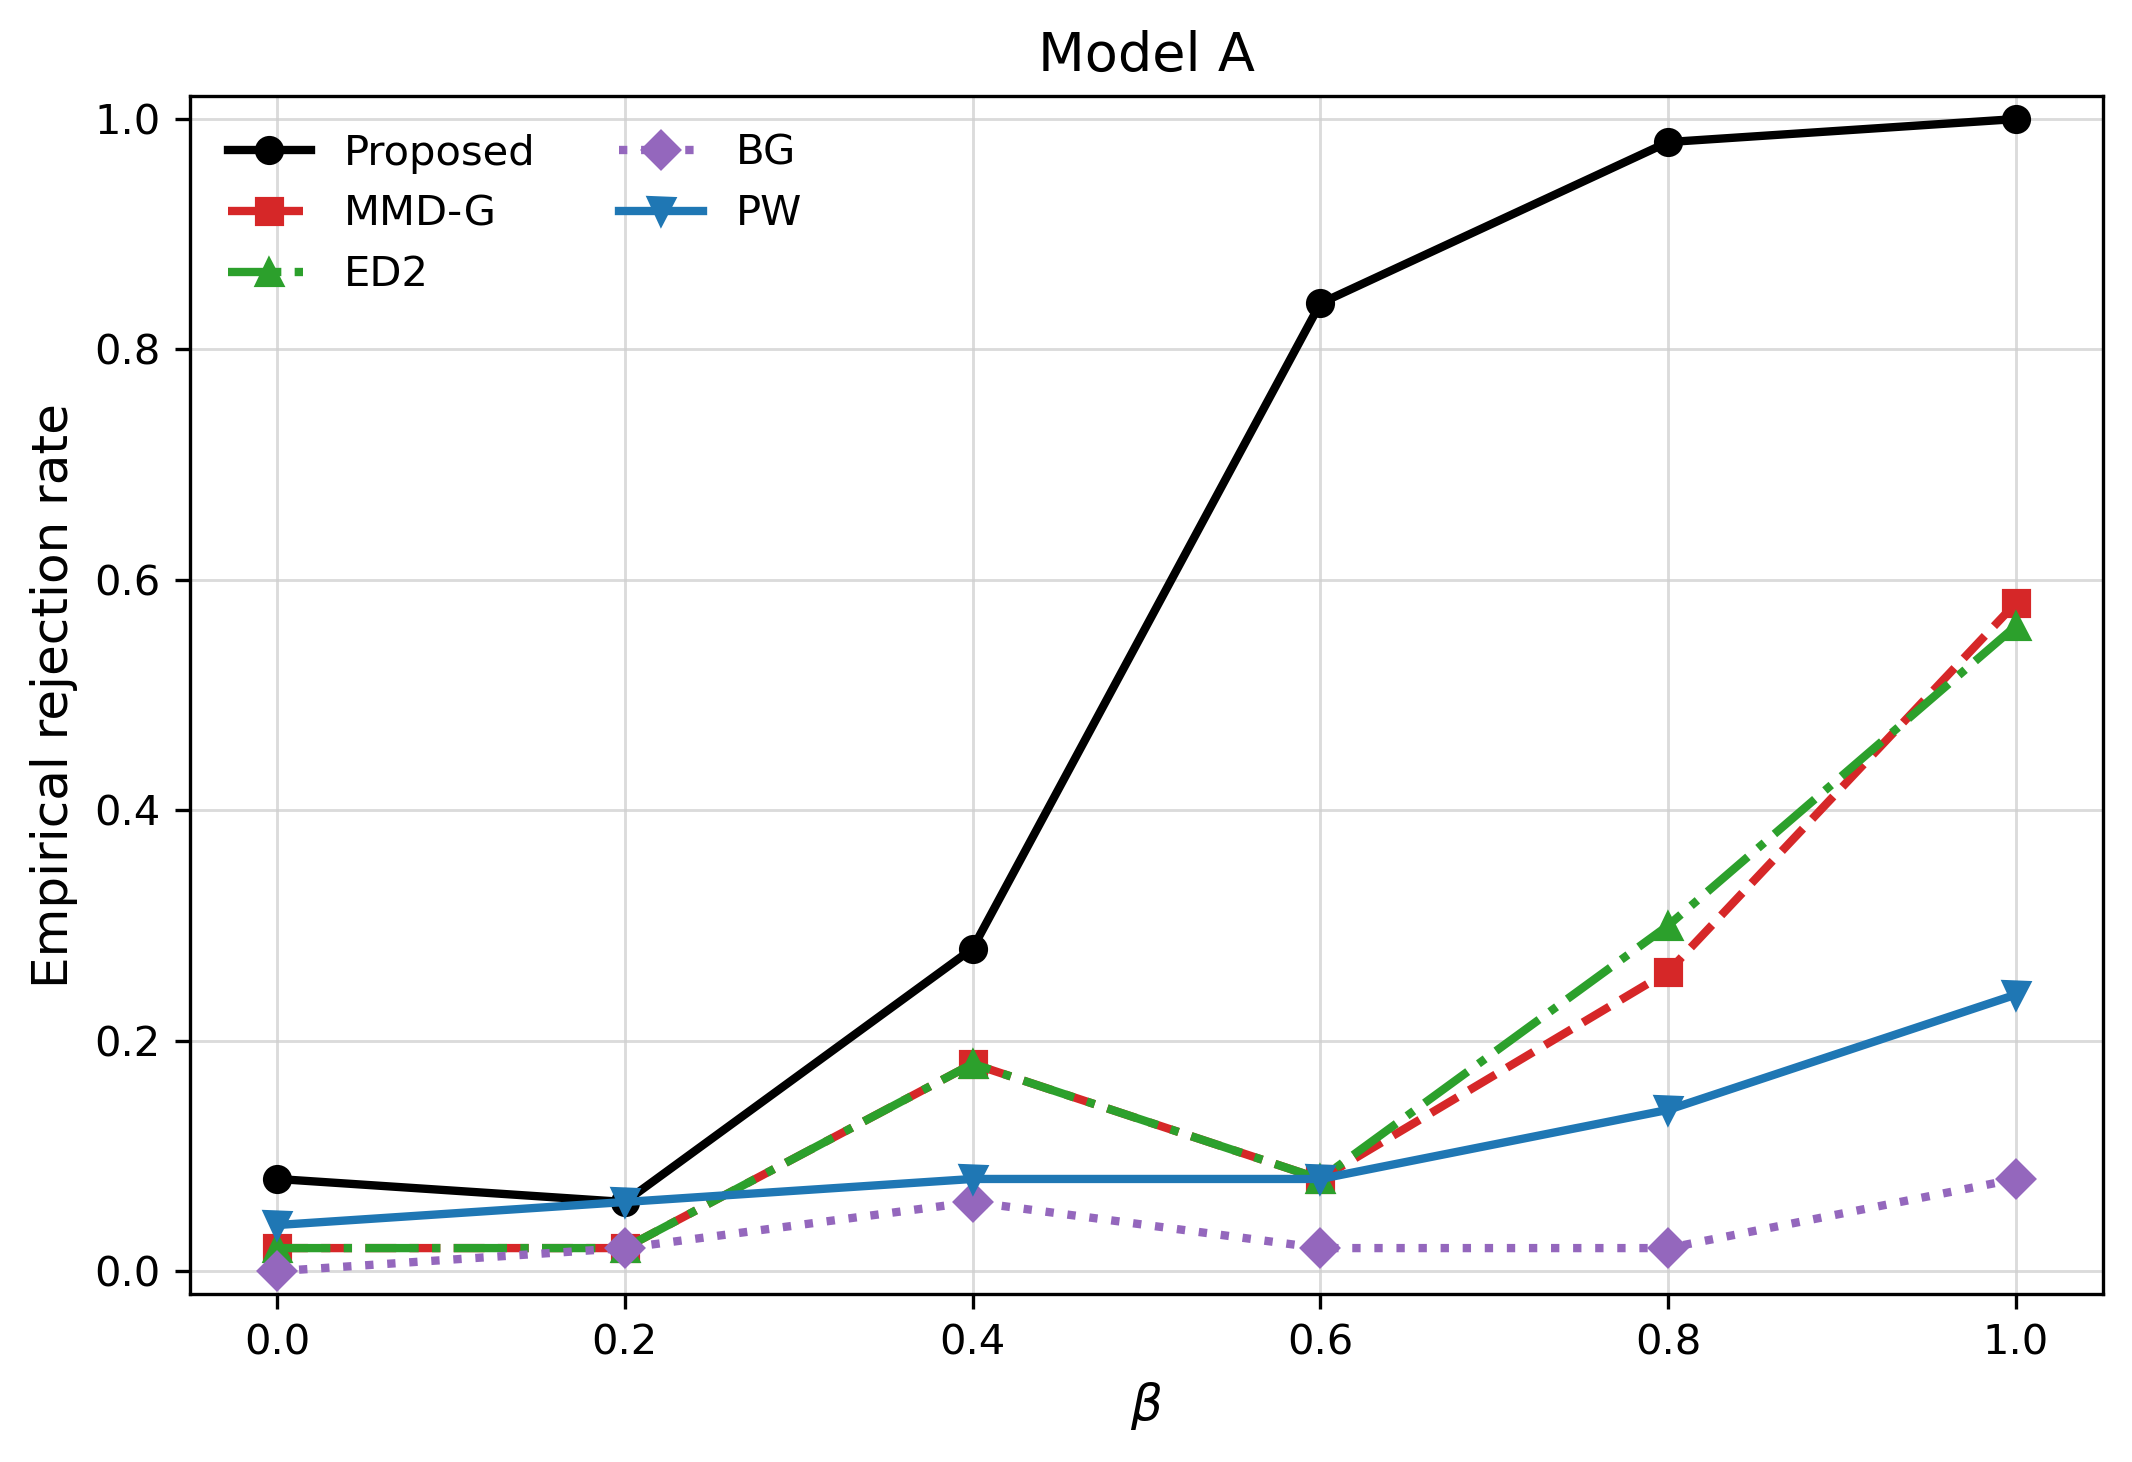
\includegraphics[width=0.88\textwidth]{../Fig1-ModelA/Figure1_ModelA_first50.png}
\caption{Model A 下不同方法的经验拒绝率。每个 \(\beta\) 只使用前 50 个完整轮次。}
\label{fig:modela}
\end{figure}

\section{结果解读}

当 \(\beta=0\) 时，两组分布在数据生成机制下没有均值差异，此时经验拒绝率反映 size
控制情况。五种方法在 \(\beta=0\) 下的拒绝率均较低，其中 Proposed 为 0.08，略高于
显著性水平 0.05，但由于这里只使用 50 轮模拟，存在一定 Monte Carlo 波动。

随着 \(\beta\) 增大，Proposed 方法的经验拒绝率快速上升：在 \(\beta=0.4\) 时为
0.28，在 \(\beta=0.6\) 时达到 0.84，并在 \(\beta=0.8\) 和 \(\beta=1.0\) 时接近或达到
1。这说明在当前 Model A 的稀疏衰减均值差异下，Proposed 方法对信号增强非常敏感。

相比之下，MMD-G 与 ED2 也随 \(\beta\) 增大而上升，但整体功效低于 Proposed；在
\(\beta=1.0\) 时分别为 0.58 和 0.56。BG 与 PW 的拒绝率整体较低，说明它们在该高维、
坐标衰减的均值差异场景下检测能力相对有限。

总体来看，本次复现实验支持论文 Figure 1 中 Model A 的主要现象：在高维稀疏或衰减型
均值差异下，基于 max-sliced Wasserstein distance 的 Proposed 方法具有明显更强的检测功效。

\end{document}
